\documentclass[12pt, titlepage]{article}
\usepackage[swedish]{babel}
\usepackage[margin=2.5cm]{geometry}
\usepackage[style=authoryear, backend=biber, maxcitenames=3, maxbibnames=99,  giveninits=true, uniquename=init]{biblatex}
\usepackage[T1]{fontenc}
\usepackage[utf8]{inputenc}
\urlstyle{same}
\usepackage{xurl}
\usepackage{newtxtext, newtxmath, graphicx, hyperref}
\usepackage{setspace, amsmath, amssymb, amsthm}
\usepackage{float, fancyhdr, enumitem}
\usepackage{booktabs, tabularx, multicol, multirow}
\usepackage{caption, changepage, array, titlesec}
\setlength{\parindent}{0pt}
\pagestyle{fancy}
\fancyhf{}
\rhead{\thepage}
\renewcommand{\headrulewidth}{0pt}
\addbibresource{sample.bib}
\usepackage{float}       % For the [H] placement specifier
\usepackage{tikz}        % Required for TikZ
\usepackage{pgfplots}    % Required for axis, addplot, etc.
\pgfplotsset{compat=newest}  % Recommended for PGFPlots
\usepackage{pgfplotstable}
\usetikzlibrary{patterns}    % Required for pattern fills
\usepackage{xcolor}
\definecolor{darkblue}{RGB}{0,0,120}



\onehalfspacing



\titleformat{\section}
  {\normalfont\fontsize{16}{18}\bfseries}
  {\thesection}
  {1em}
  {}
\titleformat{\subsection}
  {\normalfont\fontsize{14}{16}\bfseries}
  {\thesubsection}
  {1em}
  {}
\titleformat{\subsubsection}
  {\normalfont\fontsize{12}{14}\bfseries}
  {\thesubsubsection}
  {1em}
  {}
\setcounter{secnumdepth}{3}
\setcounter{tocdepth}{3}


\title{Skatt -- Belgien}
\author{
    Grupp 41 \\ \\
    Aron Dovrén\\
    Timur Armak\\
    Yunshan Luo\\
    Alexander Järvheden \\
}
\date{}
\begin{document}
\maketitle
\newpage
\tableofcontents
\newpage

\section{Introduktion}
    \subsection{Bakgrund} 
    %Lite snack om Belgien och deras skatt

    Belgien är det land i Europa som ofta lyfts fram för sitt höga skattesystem. Under lång tid har landet haft ett av Europas högsta skattetryck, där de totala skatteintäkterna motsvarat ungefär 44--48\;\% av BNP enligt Eurostats datatabell 
    \textit{gov\_10a\_taxag} \parencite{eurostat_taxgdp}. Skattesystemet kännetecknas av en tung beskattning av arbete, särskilt genom höga sociala avgifter och en omfattande skattekil. Enligt OECD har Belgien även den högsta skattekilen i Europa, vilket innebär att en stor del av arbetskraftskostnaden går till skatter och avgifter snarare än nettolön \parencite{oecd_taxingwages}. 
    Sammantaget gör detta Belgien till ett relevant fall för att analysera olika typer av skattenyckeltal och korrelationen mellan skatt och sysselsättningsgrad samt en jämförelse med Sveriges skattesituation. 


    \subsection{Problemformulering}
    %Vad vill vi analysera?  idk

    Denna rapport syftar till att analysera nyckeldata inom området skatt. 
    
    Fokusområde har varit:
    \begin{itemize}
        \item Samlat skattetryck,
        \item Skatteintäkter fördelat på skattebaser,
        \item Lafferkurva,
        \item Korrelation mellan skatt och arbetsutbud.
    \end{itemize}
 
    \subsection{Syfte och Frågeställning}
    Rapportens syfte är att analysera Belgiens skattetryck och dess relation till landets skatteintäkter och arbetskraftsbeskattning. Målet är att identifiera Belgiens position på Lafferkurvan samt att undersöka hur denna position förhåller sig till andra europeiska länder. Genom att kombinera Eurostats skattetrycksdata med OECD:s mått på skattekil och arbetsmarknadsutfall avser studien att belysa hur skattesystemets utformning kan påverka arbetsutbud och skatteintäkter.

Mot bakgrund av detta formuleras följande frågeställningar:

\begin{itemize}
    \item Hur har Belgiens skattetryck och skatteintäkter utvecklats under perioden 2017--2024?
    \item Vilken position indikerar Belgien att ha på Lafferkurvan baserat på tillgängliga data?
    \item Hur skiljer sig Belgiens skattetryck och skattekil från Sverige?
    \item Vilka potentiella effekter kan skattesystemet ha på arbetsutbud och sysselsättningsgrad?
\end{itemize} 

\section{Metod och Material}

    \subsection{Dataset och Urval}
    %Förklara vilka källor/dataset vi har valt och varför
    I studien används huvudsakligen offentligt tillgängliga makroekonomiska dataset från Eurostat och OECD, samt kompletterande demografisk statistik från SCB. Eurostats databaser tillhandahåller information om bland annat skattetryck \parencite{eurostat_taxgdp} och arbetsmarknadsvariabler såsom sysselsättningsgrad. OECD:s databaser används för att hämta information om skattekilen (tax wedge) och arbetskraftsbeskattning, vilka fungerar som centrala indikatorer för att analysera hur skattesystemet påverkar arbetsutbud och skatteintäkter. SCB:s databas har använts för att hämta relevanta data för svenska nyckeltal. Dessa källor valdes eftersom de erbjuder internationellt jämförbara mått med hög reliabilitet och är offentligt tillgängliga. 

    \subsection{Analysmetoder och Koncept}
    Rapporten fokuserar på deskriptiv analys som tillämpar kvantitativ analys med nationalekonomisk teori. Dessutom används en komparativ analys som komplement, där Belgiens data ställs i jämförelse med Sveriges. 
    \newline

    För att undersöka sambandet mellan skatt och arbete används en Pearson-korrelationsanalys mellan den årliga skatteprocenten och sysselsättningsgraden. Denna analys syftar till att identifiera om det finns ett statistiskt säkerställt samband mellan sänkningar i skattetrycket och ökad sysselsättning. Lafferkurvan modelleras utifrån teorin och nyckeltalen givna i arbetspappret av Jacob Lundberg \parencite{lundberg2017laffer}.

    \subsubsection{Metoder, Modeller och Nyckeltal}

    I analysen används följande centrala metoder och begrepp:

    
    \paragraph{Skattetryck (Tax-to-GDP Ratio):}

    Skattetrycket definieras som de totala skatteintäkterna i relation till BNP och används som ett övergripande mått på skattesystemets storlek. Data hämtas från Eurostats datatabell \textit{gov\_10a\_taxag} \parencite{eurostat_taxgdp}.
    
    \paragraph{Skattekil (Tax Wedge):}
    Skattekilen mäter skillnaden mellan arbetsgivarens totala arbetskraftskostnad och arbetstagarens nettolön. Måttet inkluderar inkomstskatt samt både arbetsgivar- och arbetstagaravgifter och används för att fånga arbetskraftens effektiva beskattning. Värden hämtas från OECD:s och Eurostats indikator \textit{earn\_nt\_taxwedge} \parencite{eurostat_taxwedge}.
    
    \paragraph{Lafferkurvan:}
    Lafferkurvan beskriver sambandet mellan skattesats och skatteintäkter och illustrerar att intäkterna ökar upp till en optimal nivå innan de minskar vid för höga skattesatser. I rapporten modelleras Lafferkurvan genom ett teoretiskt resonemang i ett nationalekonomiskt ramverk.\parencite{lundberg2017laffer}
    
    \paragraph{Komparativ analys:}
    Belgien jämförs med Sverige för att illustrera skillnader i skattesystemens struktur och arbetsmarknadsutfall. Denna jämförelse fungerar som ett referensramverk för att bedöma hur Belgien positionerar sig i en europeisk kontext.%källa

    \paragraph{AD/AS-modellen:}
    Används för att visa hur skatteförändringar påverkar den aggregerade efterfrågan och det aggregerade utbudet i ekonomin.

    \subsection{Antaganden och Avgränsningar}

        \subsubsection{Avgränsningar}
        För att arbetet inte ska bli för omfattande har rapporten avgränsats till perioden 2017 och framåt för skattenyckeltalen. Vid beräkningarna av sysselsättningsgraden avgränsar rapporten sig från 2015 och framåt samt mellan åldrarna 20-64 då data för övriga åldrar kan missleda analysen med motivationen att man, mellan åldrarna 15-19 och 65+, går i skola eller är pensionerad. Analysen tar inte hänsyn till inflation, konjunkturer eller förändringar i BNP:s sammansättning. Rapporten utgår även från att Eurostats och OECD:s indikatorer är enhetliga och direkt jämförbara mellan år. Vidare analyseras enbart nationella genomsnitt, vilket innebär att regionala skillnader inom Belgien inte beaktas.
        \\

        Analysen avgränsas till de tre huvudsakliga skattebaserna: arbete, kapital och konsumtion. Detta val motiveras främst av att dessa kategorier tillsammans utgör den totala majoriteten av Belgiens totala skatteintäkter, där skatten på arbete står för över hälften av de samlade skatteintäkterna. Genom att fokusera på dessa tre huvudposter säkerställs att analysen täcker de delar av skattesystemet som har störst påverkan på landets ekonomi och invånarnas beteende. Vidare görs denna avgränsning för att hålla arbetet inom en rimlig omfattning och möjliggöra en djupare diskussion kring de mest betydelsefulla incitamentseffekterna, snarare än en ytlig genomgång av samtliga mindre skatteposter.
    

        \subsubsection{Antaganden}
        För att kunna modellera den belgiska Lafferkurvan och analysera dess effekter krävs vissa antaganden kring ekonomins struktur. I denna rapport används de nyckeltal som identifierats av \cite{lundberg2017laffer}, vilka anses vara relevanta för analysen av följande skäl:
        
        \begin{itemize}
            \item \textbf{Paretoparametern ($\alpha = 2,03$):} Denna siffra beskriver inkomstfördelningen i toppen av inkomstskalan. Ett lands grundläggande inkomststruktur, det vill säga hur inkomsterna är fördelade mellan olika grupper. Detta är en fundamental egenskap i ekonomin som förändras mycket långsamt över tid. Trots att Lundbergs studie publicerades 2017 bedöms värdet för Belgien fortfarande vara representativt för dagens förhållanden då inga drastiska strukturella skiften i inkomstfördelningen observerats.
            
            \item \textbf{Elasticiteten ($\varepsilon = 0,2$):} Elasticiteten mäter hur känsligt arbetsutbudet och den beskattningsbara inkomsten är för förändringar i skattesatsen. Ett värde på $0,2$ är en etablerad standard inom internationell ekonomisk forskning och betraktas som ett konservativt och försiktigt antagande. Genom att använda detta värde undviker man att överskatta effekterna av skatteförändringar, vilket ger analysen en högre grad av trovärdighet.
        \end{itemize}

\section{Resultat och Deskriptiv Analys}
    \subsection{Det samlade skattetrycket Belgien}
     %visa skattekvot, och eventuell jämförelse med andra/annat EU-land\\
    \begin{table}[H]
    \centering
    \label{tab:belgien_bnp}
    \vspace{0.2cm} % Lite extra mellanrum mellan caption och tabell
    \begin{tabular}{lrrr} % l=left för år, r=right för siffror så de står snyggt
        \toprule
        \textbf{År} & \textbf{BNP (miljoner euro)} & \textbf{Skatteintäkter (miljoner euro)} & \textbf{Skattetryck} \\
        \midrule
        2017 & 428 467,1 & 209 513,8 & 47,3 \% \\
        2018 & 443 407,2 & 216 697,0 & 47,2 \% \\
        2019 & 459 491,8 & 218 578,4 & 45,6 \% \\
        2020 & 479 444,9 & 210 837,2 & 45,5 \% \\
        2021 & 463 750,9 & 230 205,7 & 45,5 \% \\
        2022 & 506 047,2 & 251 272,5 & 44,8 \% \\
        2023 & 561 309,1 & 267 590,2 & 44,4 \% \\
        2024 & 602 376,3 & 279 744,8 & 45,1 \% \\
        \bottomrule
    \end{tabular}
    \caption{Belgiens BNP och skatteintäkter 2017–2024}
    \end{table}
    
     \subsection{Det samlade skattetrycket Sverige}
    \begin{table}[H]
    \centering
    \label{tab:sverige_bnp}
    \vspace{0.2cm} % Lite extra mellanrum mellan caption och tabell
    \begin{tabular}{lrrr} % l=left för år, r=right för siffror så de står snyggt
        \toprule
        \textbf{År} & \textbf{BNP (miljoner kr)} & \textbf{Skatteintäkter (miljoner kr)} & \textbf{Skattetryck} \\
        \midrule
        2017 & 4 575 114 & 2 039 152 & 45 \% \\
        2018 & 4 777 837 & 2 113 857 & 44 \% \\
        2019 & 5 021 382 & 2 162 925 & 43 \% \\
        2020 & 5 012 855 & 2 137 949 & 43 \% \\
        2021 & 5 417 760 & 2 336 817 & 43 \% \\
        2022 & 5 816 415 & 2 493 410 & 43 \% \\
        2023 & 6 143 187 & 2 562 206 & 42 \% \\
        2024 & 6 387 027 & 2 643 673 & 41 \% \\
        \bottomrule
    \end{tabular}
    \caption{Sveriges BNP och skatteintäkter 2017–2024}
    \end{table}

\newpage
    \subsection{Fördelning av skattebaser}
        %Visa vart skatteintäkter kommer ifrån och hur mycket från respektive del (arbete, konsumtion, kapital osv.).
        
        \subsubsection{Belgiens fördelning på skattebaser}
        
        \begin{table}[H]
        \centering
        \begin{tabular}{lrrr}
        \toprule
        \textbf{År} & \textbf{Konsumtion (mn EUR)} & \textbf{Arbete (mn EUR)} & \textbf{Kapital (mn EUR)} \\ 
        \midrule
        2017 & 48 107 & 100 622 & 49 370 \\ 
        2018 & 49 989 & 103 044 & 51 956 \\ 
        2019 & 51 004 & 105 366 & 50 195 \\ 
        2020 & 47 272 & 105 547 & 45 539 \\ 
        2021 & 53 630 & 110 261 & 53 580 \\ 
        2022 & 55 487 & 123 776 & 58 618 \\ 
        2023 & 57 780 & 131 103 & 63 366 \\
        \bottomrule
        \end{tabular}
        \caption{Belgien: Totala skatteintäkter fördelat på skattebaser i miljoner euro.}
        \end{table}
        
        \begin{table}[H]
        \centering
        \begin{tabular}{lrrr}
        \toprule
        \textbf{År} & \textbf{Konsumtion (\;\%)} & \textbf{Arbete (\;\%)} & \textbf{Kapital (\;\%)} \\ 
        \midrule
        2017 & 24,2 & 50,6 & 24,8 \\ 
        2018 & 24,3 & 50,1 & 25,2 \\ 
        2019 & 24,6 & 50,8 & 24,2 \\ 
        2020 & 23,7 & 53,0 & 22,9 \\ 
        2021 & 24,6 & 50,5 & 24,5 \\ 
        2022 & 23,2 & 51,8 & 24,5 \\ 
        2023 & 22,8 & 51,8 & 25,0 \\ 
        \bottomrule
        \end{tabular}
        \caption{Belgien: Procentuell fördelning av totala skatteintäkter.}
        \end{table}
        
        \begin{table}[H]
        \centering
        \begin{tabular}{lrrr}
        \toprule
        \textbf{År} & \textbf{Konsumtion (\;\%)} & \textbf{Arbete (\;\%)} & \textbf{Kapital (\;\%)} \\ 
        \midrule
        2017 & 10,9 & 22,7 & 11,1 \\ 
        2018 & 10,9 & 22,4 & 11,3 \\ 
        2019 & 10,6 & 22,0 & 10,5 \\ 
        2020 & 10,2 & 22,8 & 9,8 \\ 
        2021 & 10,6 & 21,8 & 10,6 \\ 
        2022 & 9,9 & 22,0 & 10,4 \\ 
        2023 & 9,7 & 22,0 & 10,6 \\ 
        \bottomrule
        \end{tabular}
        \caption{Belgien: Skattebaser som procent av BNP.}
        \end{table}
        
        \subsubsection{Sveriges fördelning mellan skattebaser}
        
        \begin{table}[H]
        \centering
        \begin{tabular}{lrrr}
        \toprule
        \textbf{År} & \textbf{Konsumtion (mn EUR)} & \textbf{Arbete (mn EUR)} & \textbf{Kapital (mn EUR)} \\ 
        \midrule
        2017 & 58 405 & 123 279 & 29 983 \\ 
        2018 & 57 495 & 120 285 & 28 257 \\ 
        2019 & 56 939 & 118 672 & 28 662 \\ 
        2020 & 57 470 & 118 430 & 27 985 \\ 
        2021 & 63 670 & 130 051 & 36 568 \\ 
        2022 & 66 817 & 131 272 & 36 484 \\ 
        2023 & 62 662 & 127 603 & 33 702 \\ 
        \bottomrule
        \end{tabular}
        \caption{Sverige: Totala skatteintäkter fördelat på skattebaser i miljoner euro.}
        \end{table}
        
        \begin{table}[H]
        \centering
        
        \begin{tabular}{lrrr}
        \toprule
        \textbf{År} & \textbf{Konsumtion (\;\%)} & \textbf{Arbete (\;\%)} & \textbf{Kapital (\;\%)} \\
        \midrule
        2017 & 27,6 & 58,2 & 14,2 \\ 
        2018 & 27,9 & 58,4 & 13,7 \\ 
        2019 & 27,9 & 58,1 & 14,0 \\
        2020 & 28,2 & 58,1 & 13,7 \\ 
        2021 & 27,7 & 56,5 & 15,9 \\ 
        2022 & 28,5 & 56,0 & 15,6 \\ 
        2023 & 28,0 & 57,0 & 15,1 \\ 
        \bottomrule
        \end{tabular}
        \caption{Sverige: Procentuell fördelning av totala skatteintäkter.}
        \end{table}
        
        \begin{table}[H]
        \centering
        
        \begin{tabular}{lrrr}
        \toprule
        \textbf{År} & \textbf{Konsumtion (\;\%)} & \textbf{Arbete (\;\%)} & \textbf{Kapital (\;\%)} \\ 
        \midrule
        2017 & 12,3 & 25,9 & 6,3 \\ 
        2018 & 12,3 & 25,8 & 6,1 \\ 
        2019 & 12,0 & 25,0 & 6,0 \\ 
        2020 & 12,0 & 24,7 & 5,8 \\ 
        2021 & 11,8 & 24,2 & 6,8 \\ 
        2022 & 12,1 & 23,8 & 6,6 \\ 
        2023 & 11,6 & 23,6 & 6,2 \\ 
        \bottomrule
        \end{tabular}
        \caption{Sverige: Skattebaser som procent av BNP.}
        \end{table}
    
            
                    
    \subsection{Resultat: Skattekil, sysselsättning och arbetade timmar}

Nedan presenteras den sammanställda datan för Belgien och Sverige under perioden 2015–2023. Tabellerna inkluderar skattekil, sysselsättningsgrad och det genomsnittliga antalet arbetade timmar per person.

    % Tabell 1: Belgien
    \begin{table}[ht]
    \centering
    \begin{tabular}{@{}cccc@{}}
    \toprule
    \textbf{År} & \textbf{Skattekil (\%)} & \textbf{Sysselsättningsgrad (\%)} & \textbf{Arbetade timmar} \\ \midrule
    2015        & 49,4                   & 67,2                             & 1 582                    \\
    2016        & 47,5                   & 67,7                             & 1 582                    \\
    2017        & 47,3                   & 68,5                             & 1 584                    \\
    2018        & 46,1                   & 69,7                             & 1 588                    \\
    2019        & 45,5                   & 70,5                             & 1 587                    \\
    2020        & 45,4                   & 69,7                             & 1 459                    \\
    2021        & 45,7                   & 70,6                             & 1 551                    \\
    2022        & 46,3                   & 71,9                             & 1 590                    \\
    2023        & 45,9                   & 72,1                             & 1 593                    \\ \bottomrule
    \end{tabular}
    \caption{Data för Belgien: Skattekil, sysselsättningsgrad och genomsnittligt arbetade timmar per person.}
    \label{tab:belgien_full}
    \end{table}
    
    % Tabell 2: Sverige
    \begin{table}[ht]
    \centering
    \begin{tabular}{@{}cccc@{}}
    \toprule
    \textbf{År} & \textbf{Skattekil (\%)} & \textbf{Sysselsättningsgrad (\%)} & \textbf{Arbetade timmar} \\ \midrule
    2015        & 40,6                   & 80,1                             & 1 466                    \\
    2016        & 40,8                   & 80,8                             & 1 478                    \\
    2017        & 40,9                   & 81,4                             & 1 465                    \\
    2018        & 41,0                   & 82,0                             & 1 465                    \\
    2019        & 40,5                   & 81,7                             & 1 451                    \\
    2020        & 40,5                   & 80,2                             & 1 422                    \\
    2021        & 39,8                   & 80,4                             & 1 441                    \\
    2022        & 39,5                   & 82,0                             & 1 436                    \\
    2023        & 39,8                   & 82,6                             & 1 431                    \\ \bottomrule
    \end{tabular}
    \caption{Data för Sverige: Skattekil, sysselsättningsgrad och genomsnittligt arbetade timmar per person}
    \label{tab:sverige_full}
    \end{table}
    

    \newpage
    \subsection{Sambandet i siffror}
% \begin{tikzpicture}
% \pgfplotsset{
%     scale only axis,
%     scaled x ticks=base 10:3,
%     xmin=0, xmax=0.06
% }

% \begin{axis}[
%   axis y line*=left,
%   ymin=0, ymax=80,
%   xlabel=År,
%   ylabel=Procent \%,
% ]
% \addplot[smooth,mark=x,red]
%   coordinates{
% (2017,40.9)
% (2018,41.0)
% (2019,40.5)
% (2020,40.5)
% (2021,39.8)
% (2022,39.5)
% (2023,39.8)
% }; \label{plot_one}

% \addplot[smooth,mark=o,green]
%   coordinates{
% (2017,81.4)
% (2018,82.0)
% (2019,81.7)
% (2020,80.2)
% (2021,80.4)
% (2022,82.0)
% (2023,82.6)
% }; \label{plot_two}

% \end{axis}

% \begin{axis}[
%   axis y line*=right,
%   axis x line=none,
%   ymin=0, ymax=100,
%   ylabel=Arbetade timmar ($h$) per person 
% ]
% \addlegendimage{/pgfplots/refstyle=plot_one}\addlegendentry{Skattekil}
% \addlegendimage{/pgfplots/refstyle=plot_two}\addlegendentry{Sysselsättningsgrad}
% \addplot[smooth,mark=*,blue]
%   coordinates{
% (2017,1465)
% (2018,1465)
% (2019,1451)
% (2020,1422)
% (2021,1441)
% (2022,1436)
% (2023,1431)
% }; \addlegendentry{Arbetade timmar}
% \end{axis}

% \end{tikzpicture}

\begin{figure}[ht!]
    \centering
    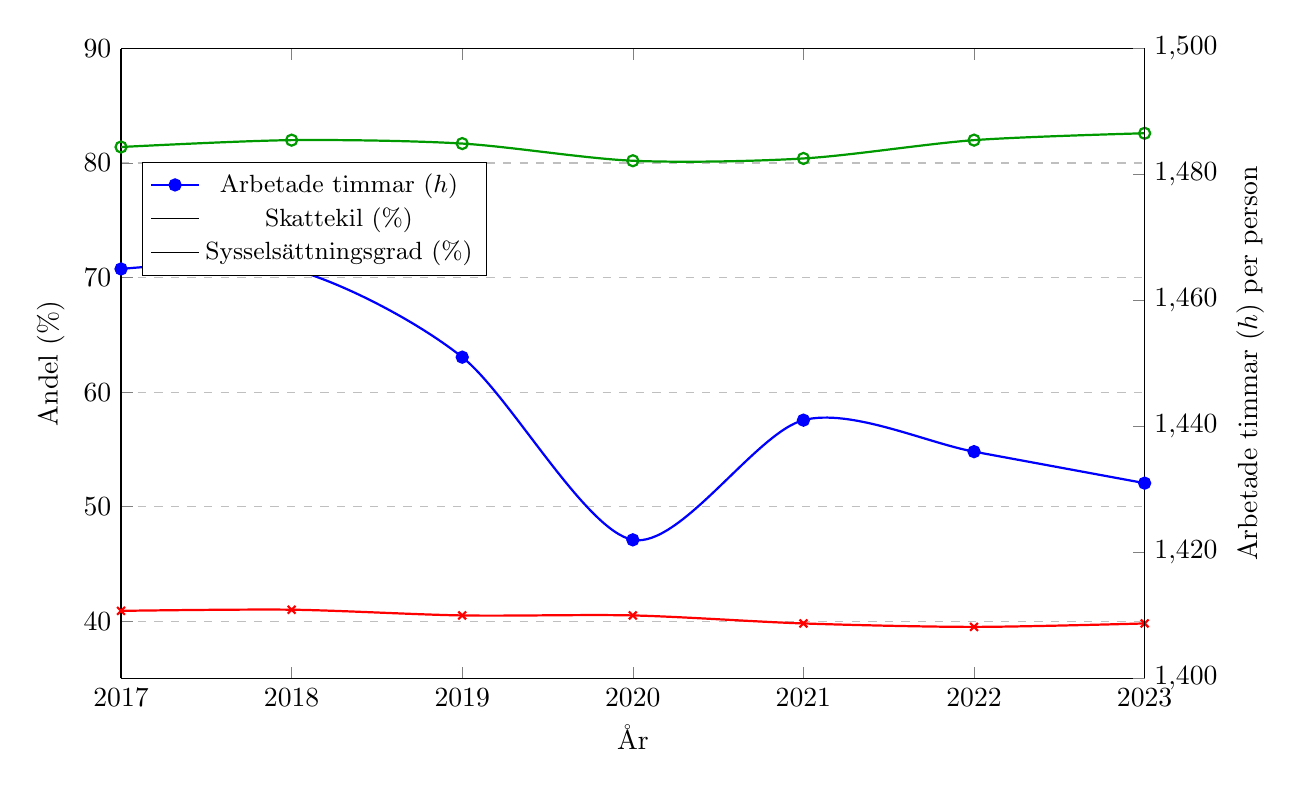
\begin{tikzpicture}
\pgfplotsset{
    width=13cm,
    height=8cm,
    scale only axis,
    xmin=2017, xmax=2023,
    xtick={2017,2018,...,2023},
    x tick label style={/pgf/number format/1000 sep={}} % Tar bort tusentalsavgränsare i årtal
}

\begin{axis}[
  axis y line*=left,
  ymin=35, ymax=90, % Justerat för att rymma både ~40% och ~80%
  xlabel={År},
  ylabel={Andel (\%)},
  ymajorgrids=true,
  grid style=dashed,
  % legend style={at={(0.02,0.98)}, anchor=north west, font=\small}
]
% Skattekil
\addplot[smooth, thick, mark=x, red]
  coordinates{
    (2017,40.9) (2018,41.0) (2019,40.5) (2020,40.5) (2021,39.8) (2022,39.5) (2023,39.8)
  }; \label{plot_skattekil}

% Sysselsättningsgrad
\addplot[smooth, thick, mark=o, green!60!black]
  coordinates{
    (2017,81.4) (2018,82.0) (2019,81.7) (2020,80.2) (2021,80.4) (2022,82.0) (2023,82.6)
  }; \label{plot_sysselsattning}
\end{axis}

\begin{axis}[
  axis y line*=right,
  axis x line=none,
  ymin=1400, ymax=1500, % Justerat för att passa arbetade timmar (~1450)
  ylabel={Arbetade timmar ($h$) per person},
  legend style={at={(0.02,0.82)}, anchor=north west, font=\small}
]
% Arbetade timmar
\addplot[smooth, thick, mark=*, blue]
  coordinates{
    (2017,1465) (2018,1465) (2019,1451) (2020,1422) (2021,1441) (2022,1436) (2023,1431)
  }; \label{plot_timmar}

% Samlad legend i den högra axelns miljö (valfritt, men snyggt)
\addlegendimage{/pgfplots/refstyle=plot_skattekil}\addlegendentry{Arbetade timmar ($h$)}
\addlegendimage{/pgfplots/refstyle=plot_sysselsattning}\addlegendentry{Skattekil (\%)}
\addlegendimage{/pgfplots/refstyle=plot_timmar}\addlegendentry{Sysselsättningsgrad (\%)}
\end{axis}

\end{tikzpicture}
    \caption{Sveriges sysselsättningsgrad och skattekil (vänster axel), arbetade timmar per person (höger axel) utveckling mellan 2017 och 2023}
    \label{fig:placeholder}
\end{figure}

% \begin{figure}[ht!]
%     \centering
%     \begin{tikzpicture}
% \pgfplotsset{
%     width=13cm,
%     height=8cm,
%     scale only axis,
%     xmin=2017, xmax=2023,
%     xtick={2017,2018,...,2023},
%     x tick label style={/pgf/number format/1000 sep={}} % Tar bort tusentalsavgränsare i årtal
% }

% \begin{axis}[
%   axis y line*=left,
%   ymin=35, ymax=90, % Justerat för att rymma både ~40% och ~80%
%   xlabel={År},
%   ylabel={Andel (\%)},
%   ymajorgrids=true,
%   grid style=dashed,
%   legend style={at={(0.02,0.98)}, anchor=north west, font=\small}
% ]
% % Skattekil
% \addplot[smooth, thick, mark=x, red]
%   coordinates{
%     (2017,47.3) (2018,46.1) (2019,45.5) (2020,45.4) (2021,45.7) (2022,46.3) (2023,45.9)
%   }; \label{plot_skattekil2}

% % Sysselsättningsgrad
% \addplot[smooth, thick, mark=o, green!60!black]
%   coordinates{
%     (2017,68.5) (2018,69.7) (2019,70.5) (2020,69.7) (2021,70.6) (2022,71.9) (2023,72.1)
%   }; \label{plot_sysselsattning2}
% \end{axis}

% \begin{axis}[
%   axis y line*=right,
%   axis x line=none,
%   ymin=1400, ymax=1500, % Justerat för att passa arbetade timmar (~1450)
%   ylabel={Arbetade timmar ($h$) per person},
%   legend style={at={(0.02,0.82)}, anchor=north west, font=\small}
% ]
% % Arbetade timmar
% \addplot[smooth, thick, mark=*, blue]
%   coordinates{
%     (2017,1584) (2018,1588) (2019,1587) (2020,1459) (2021,1551) (2022,1590) (2023,1593)
%   }; \label{plot_timmar2}

% % Samlad legend i den högra axelns miljö (valfritt, men snyggt)
% \addlegendimage{/pgfplots/refstyle=plot_timmar2}\addlegendentry{Arbetade timmar ($h$)}
% \addlegendimage{/pgfplots/refstyle=plot_skattekil2}\addlegendentry{Skattekil (\%)}
% \addlegendimage{/pgfplots/refstyle=plot_sysselsattning2}\addlegendentry{Sysselsättningsgrad (\%)}
% \end{axis}

% \end{tikzpicture}
%     \caption{Belgiens sysselsättningsgrad och skattekil (vänster axel), arbetade timmar per person (höger axel) utveckling mellan 2017 och 2023}
%     \label{fig:placeholder}
% \end{figure}

\begin{figure}[ht!]
    \centering
    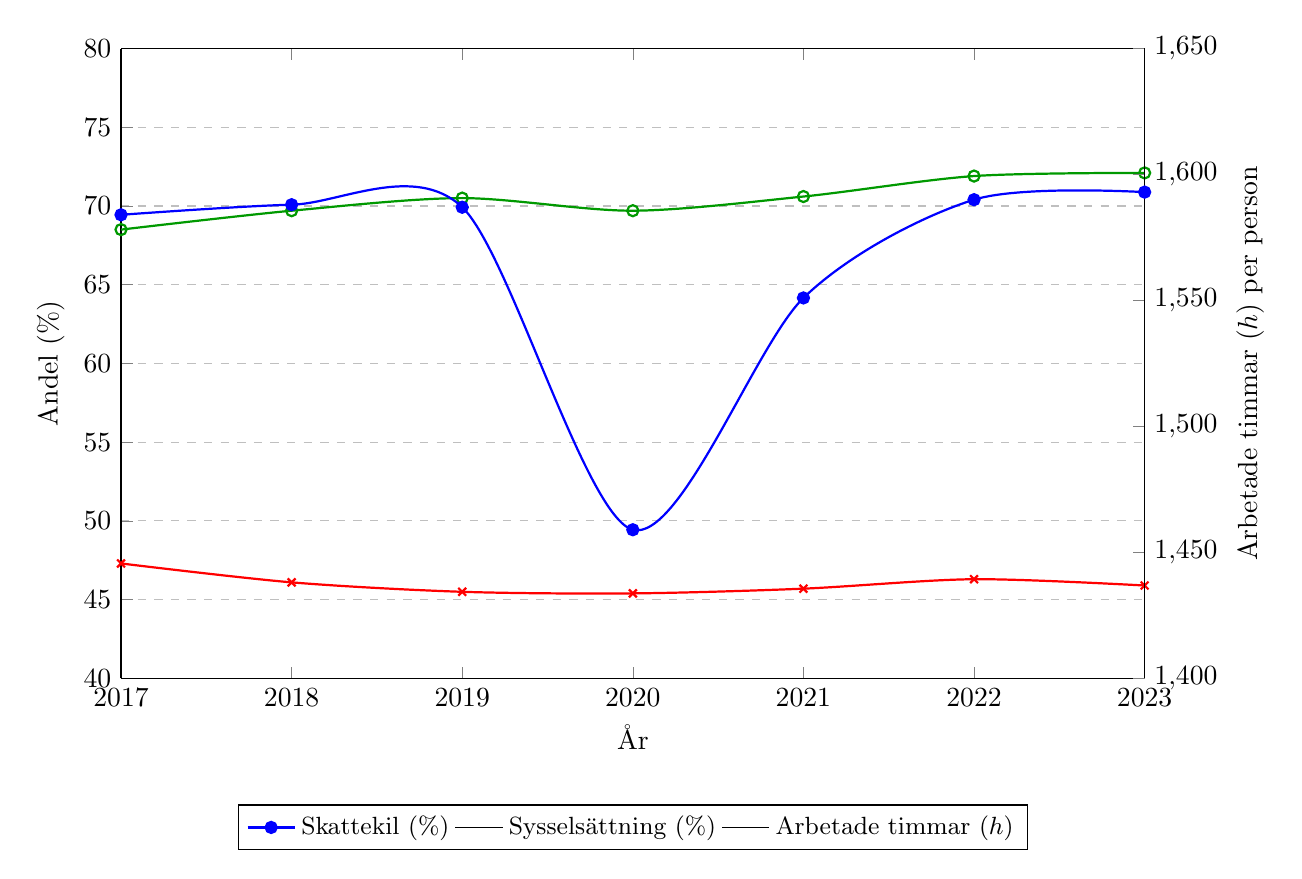
\begin{tikzpicture}
\pgfplotsset{
    width=13cm,
    height=8cm,
    scale only axis,
    xmin=2017, xmax=2023,
    xtick={2017,2018,...,2023},
    x tick label style={/pgf/number format/1000 sep={}} 
}

\begin{axis}[
  axis y line*=left,
  ymin=40, ymax=80, % Optimerat för Belgien (45% och 70%)
  xlabel={År},
  ylabel={Andel (\%)},
  ymajorgrids=true,
  grid style=dashed,
]
% Skattekil
\addplot[smooth, thick, mark=x, red]
  coordinates{
    (2017,47.3) (2018,46.1) (2019,45.5) (2020,45.4) (2021,45.7) (2022,46.3) (2023,45.9)
  }; \label{plot_skattekil_be}

% Sysselsättningsgrad
\addplot[smooth, thick, mark=o, green!60!black]
  coordinates{
    (2017,68.5) (2018,69.7) (2019,70.5) (2020,69.7) (2021,70.6) (2022,71.9) (2023,72.1)
  }; \label{plot_sysselsattning_be}
\end{axis}

\begin{axis}[
  axis y line*=right,
  axis x line=none,
  ymin=1400, ymax=1650, % Korrigerat för att rymma värden upp till 1593
  ylabel={Arbetade timmar ($h$) per person},
  legend style={at={(0.5,-0.2)}, anchor=north, legend columns=3, font=\small} % Placerad under grafen för tydlighet
]
% Arbetade timmar
\addplot[smooth, thick, mark=*, blue]
  coordinates{
    (2017,1584) (2018,1588) (2019,1587) (2020,1459) (2021,1551) (2022,1590) (2023,1593)
  }; \label{plot_timmar_be}

% Samlad legend
\addlegendimage{/pgfplots/refstyle=plot_skattekil_be}\addlegendentry{Skattekil (\%)}
\addlegendimage{/pgfplots/refstyle=plot_sysselsattning_be}\addlegendentry{Sysselsättning (\%)}
\addlegendimage{/pgfplots/refstyle=plot_timmar_be}\addlegendentry{Arbetade timmar ($h$)}
\end{axis}

\end{tikzpicture}
    \caption{Belgiens sysselsättningsgrad och skattekil (vänster axel), arbetade timmar per person (höger axel) utveckling mellan 2017 och 2023}
    \label{fig:belgium_stats}
\end{figure}

\clearpage
    
    %Visa en fin bild som visar det vi vill visa :)

\section{Analys och Diskussion}
    \subsection{Analys av Lafferkurvan}
    Lafferkurvan illustrerar den teoretiska relationen mellan skattesatser och statens totala skatteintäkter. Lafferkurvan bygger på ett nationalekonomiskt antagande om att både för låga och för höga skattesatser ger lägre skatteintäkter än vad som anses vara optimalt. Om skattesatsen är för låg leder det till att det finns orealiserad potential för staten att finansiera välfärd, medan en för hög skattesats leder till lägre skatteintäkter som hämmar ekonomisk aktivitet och företagande. Samtidigt ger det incitament för beteendeförändringar som minskar arbetsutbudet, skatteplanering och offshoring. Detta innebär att värdeskapande verksamheter som tidigare betraktades som lönsamma inrikes måste flytta utomlands för att bevara sin lönsamhet.
    \\

Lafferkurvan modelleras enligt funktionen $$R(\tau)=N_0(\Bar{z}_b+b)\tau(1-\tau)^{\alpha\epsilon}$$

    där $\Bar{z}_b$ är den genomsnittliga inkomsten hos de största skattebetalarna. $\tau$ är den högsta marginalskatten. $b$ är tröskeln där det börjar att gälla. $\varepsilon$ är elasticitet. $\alpha$ är Paretoparemetern. $N_0$ är proportionen av skattebetalare vars inkomstpotential överstiger tröskeln $b$.
    

    \begin{figure}[H]
    \centering
    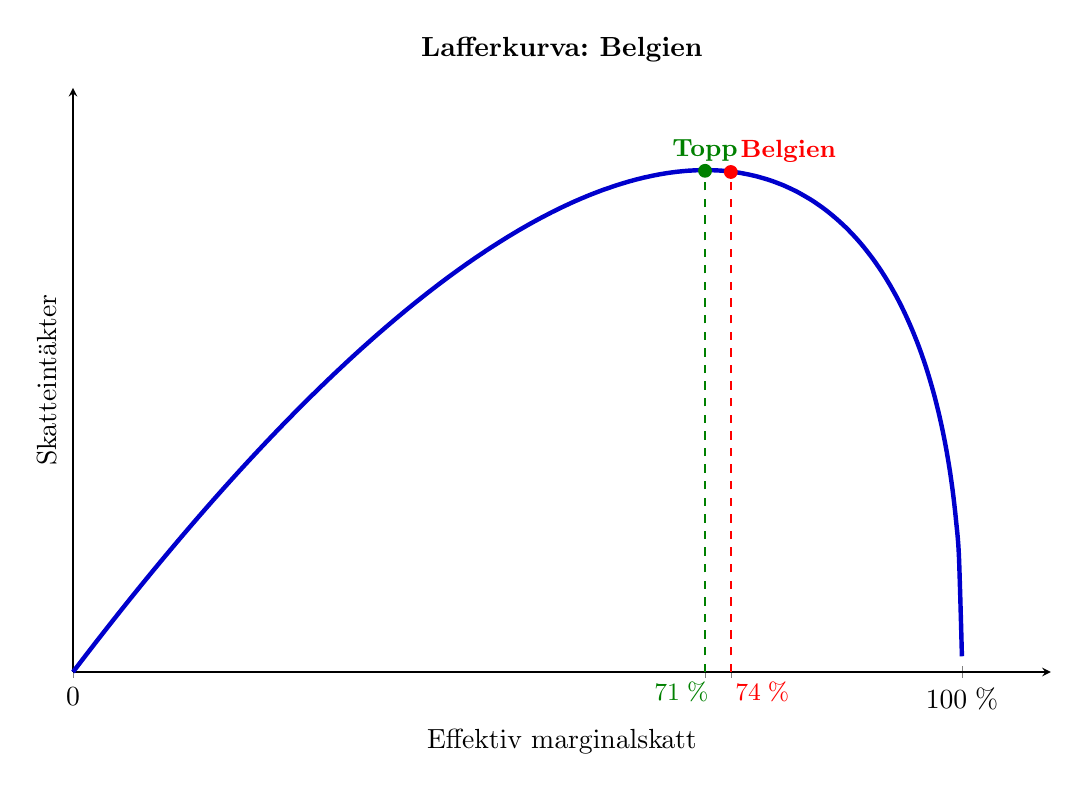
\begin{tikzpicture}
    \begin{axis}[
        axis lines = left,
        xlabel = {Effektiv marginalskatt},
        ylabel = {Skatteintäkter},
        xmin=0, xmax=1.1,
        ymin=0, ymax=0.5,
        width=14cm,  % Större bredd
        height=9cm,  % Större höjd
        % Vi sätter de exakta ticksen men döljer standardetiketterna för 71/74
        xtick={0, 0.711, 0.74, 1.0},
        xticklabels={0, , , 100\;\%}, 
        ytick=\empty,
        clip=false,
        title={\textbf{Lafferkurva: Belgien}}
    ]
        % Lafferkurvan ritas med hög upplösning
        \addplot [
            domain=0:1, 
            samples=300, 
            blue!80!black, 
            ultra thick,
            smooth
        ] {x*(1-x)^0.406};
    
        % Markera Toppen (71.1%)
        \coordinate (top) at (axis cs:0.711, 0.429);
        \draw[dashed, green!50!black, thick] (axis cs:0.711, 0) -- (top);
        \fill[green!50!black] (top) circle (2.5pt);
        
        % Manuell etikett för 71% - skjuten lite till vänster
        \node[anchor=north, color=green!50!black, xshift=-0.3cm] at (axis cs:0.711, 0) {\small 71\;\%};
        \node[anchor=south, color=green!50!black, font=\small\bfseries] at (top) {Topp};
    
        % Markera Belgien (74%)
        \coordinate (belgium) at (axis cs:0.74, 0.428);
        \draw[dashed, red, thick] (axis cs:0.74, 0) -- (belgium);
        \fill[red] (belgium) circle (2.5pt);
    
        % Manuell etikett för 74% - skjuten lite till höger för spacing
        \node[anchor=north, color=red, xshift=0.4cm] at (axis cs:0.74, 0) {\small 74\;\%};
        \node[anchor=south west, color=red, font=\small\bfseries] at (belgium) {Belgien};
    
    \end{axis}
    \end{tikzpicture}
    \caption{Modellering av Belgiens position på Lafferkurvan.}
    \label{fig:Lafferkurva}
    \end{figure}

    Genom att applicera parametrarna från \cite{lundberg2017laffer} på den belgiska ekonomin kan man se i figur \ref{fig:Lafferkurva}. att Belgien befinner sig lite för långt åt höger på kurvan. Denna slutsats dras då den intäktsmaximerande skattenivån för Belgien beräknas ligga vid en effektiv marginalskatt på cirka 71\;\%, medan Belgiens faktiska effektiva marginalskatt uppgår till 74\;\%, vilket resulterar i landets position på "fel" sida av Lafferkurvans topp.
    \\

    Detta innebär att Belgien teoretiskt sett har för hög skatt på höga inkomster och att en sänkning på dessa skulle vara självfinansierande. Självfinansieringsgraden mäter hur stor andel av ett skattebortfall (vid en skattesänkning) som återkommer genom beteendeförändringar, exempelvis genom att folk arbetar mer och deklarerar mer inkomster. Självfinansieringsgraden beräknas som $$\text{Självfinansieringsgrad} = \frac{\alpha\varepsilon\tau}{1-\tau}$$ \cite{lundberg2017laffer} uppskattar självfinansieringsgraden till 115\;\%, vilket betyder att en skattesänkning skulle expandera skattebasen mer än vad den lägre skattesatsen minskar intäkterna. Enligt formeln för självfinansieringsgrad märker vi således att när skattesatsen ökar så ökar självfinansieringsgraden ty nämnaren minskar och täljaren ökar. Det innebär vidare att en skattesänkning skulle minska självfinansieringsgraden och därmed minska andelen av ett skattebortfall som återkommer genom beteendeförändringar.

    \subsection{Beteendeeffekter av skattekil och arbetsutbud}

    Korrelationsanalysen mellan Belgiens skattekil och sysselsättningsgrad visar ett tydligt negativt samband med en Pearson-koefficient på $-0,77$. Detta innebär att perioder med en lägre skattekil — vilket inkluderar den totala skattebördan för både arbetsgivare och arbetstagare — sammanfaller med en högre sysselsättningsgrad. För att förstå denna relation kan man utgå från de beteendemönster som beskrivs av \textcite{dornbusch2018macroeconomics}, där ekonomiskt beteende påverkas av två motverkande krafter: substitutionseffekten och inkomsteffekten.
    \newline
    
    \textit{Substitutionseffekten} innebär att individer reagerar på förändrade relativa priser. I kontexten arbetsutbud innebär en lägre skattekil att nettolönen per arbetad timme ökar i förhållande till den totala arbetskostnaden, vilket gör arbete mer attraktivt än fritid. Detta fungerar på samma sätt som när högre räntor gör framtida konsumtion mer attraktiv. Applicerat på arbetsmarknaden innebär detta att en lägre skattekil stärker incitamenten att arbeta mer, vilket i Belgien återspeglas i att antalet arbetade timmar steg från 1 582 till 1 593 per person under perioden (med undantag för pandemiåret 2020).
    \newline
    
    \textit{Inkomsteffekten} verkar i motsatt riktning och innebär att en individ med högre nettolön kan uppnå samma konsumtionsnivå med mindre arbetstid. För Belgien innebär den sänkta skattekilen (från 49,4\,\% till 45,9\,\%) att hushållens disponibla inkomst ökar. Rent teoretiskt skulle detta kunna leda till att belgiska arbetstagare väljer att konsumera mer fritid och därmed sänka sitt arbetsutbud.
    \newline

    Att sysselsättningen i Belgien ökar markant (från 67,2\,\% till 72,1\,\%) när skattekilen minskar antyder att substitutionseffekten dominerar inkomsteffekten i den Belgien. Det vill säga: en lägre skattekil gör arbete relativt mer attraktivt, och denna ökade belöning väger tyngre än den ökade inkomsten som möjliggör mer fritid.

    \subsection{Skattestrukturens effekter}
    %Diskutera varför vissa saker beskattas hårdare än andra och för- och nackdelar med dessa. Vilka konsekvenser kan det få (på arbetsmarknaden eller andra marknader)?


    \subsubsection{Översikt av Belgiens skattestruktur}
    Data från Europeiska kommissionens statistikportal \parencite{ec_taxdata_2024} visar att Belgien har en mycket tydligt koncentrerad skattestruktur. Den största delen av de offentliga skatteintäkterna kommer från 
    \textit{Taxes on labour Total}, som under perioden 2017--2023 uppgår till mellan 100 och 131 miljarder euro. 
    Arbetskraftsbeskattningen utgör därmed den klart dominerande skattebasen. Därefter följer 
    konsumtionsskatter, i storleksordningen 48--58 miljarder euro per år, och kapitalskatter som varierar 
    mellan cirka 45 och 63 miljarder euro. Inom kapitalbeskattningen är det främst skatter på 
    företagsvinster och kapitalstocken som står för merparten av intäkterna, medan hushållens 
    kapitalinkomster beskattas i betydligt mindre utsträckning.

    \subsubsection{Skattesnedsvridning och elasticitet}
    Denna struktur är konsekvent teorin om skatters snedvridning (engelska: \textit{tax-induced distortion}). Enligt 
    \cite{dornbusch2018macroeconomics} påverkar skatter ekonomiskt beteende genom 
    substitutions- och inkomsteffekter, där olika skattebaser uppvisar olika grad av elasticitet beroende 
    på hur känsliga de är för förändrade incitament. Arbetskraft är mindre rörlig än kapital och därmed 
    lättare att beskatta, men detta innebär också att skatter på arbete skapar större snedvridningar. 
    Hög arbetskraftsbeskattning minskar nettolönen och förstärker substitutionseffekten, där arbete blir 
    mindre attraktivt relativt fritid, samtidigt som arbetsgivarnas kostnader ökar. Detta kan dämpa både 
    arbetsutbud och sysselsättning. Den ojämna fördelningen av arbetslöshetens konsekvenser, som 
    diskuteras i \cite{dornbusch2018macroeconomics}, förstärker dessutom betydelsen av att undvika 
    skatter som påverkar arbetsmarknaden negativt, eftersom arbetslöshet medför stora och 
    ojämnt fördelade samhällsekonomiska kostnader.
    
    \subsubsection{Framtida skatter och Barro--Ricardo-ekvivalens}
    En ytterligare teoretisk dimension som belyser skatters distorsionseffekter är den så kallade 
    Barro--Ricardo-ekvivalensen. Enligt denna teori internaliserar hushåll framtida skatter redan idag, vilket innebär att även förväntad framtida beskattning påverkar ekonomiskt beteende 
    \parencite{dornbusch2018macroeconomics}. Detta innebär att skattedistorsioner inte enbart 
    uppstår genom dagens marginalskatter, utan även genom hushållens förväntningar om framtida 
    skattehöjningar. Resonemanget förstärker därmed argumentet att skattesystemets utformning i hög 
    grad påverkar privata beslut över tid och därmed ekonomins resursallokering.

    \subsubsection{Kapitalbeskattning och investeringar}
    Kapitalbeskattningens känslighet kan också förklaras utifrån investeringslitteraturen. Som 
    \cite{dornbusch2018macroeconomics} visar påverkar skatter direkt den så kallade 
    \textit{rental cost of capital}, det vill säga kostnaden för att använda kapital i produktionen. En högre bolagsskatt höjer denna kostnad, vilket i sin tur minskar den önskade kapitalstocken och dämpar investeringarna. Eftersom kapital är mer rörligt och mer elastiskt än arbetskraft riskerar höga kapitalskatter att leda till kapitalflykt och minskade investeringar. Av denna anledning tenderar öppna ekonomier att förlita sig mindre på kapitalskatter för att undvika effektivitetsförluster och försämrad konkurrenskraft.

    \subsubsection{Konsekvenser för arbetsutbudet}
    De teoretiska resultaten från Lafferkurvan ger en god förklaring av de effekter som observerats i Belgiens deskriptiva data. Som noterats i avsnitt 3.3 har Belgiens sysselsättningsgrad ökat i takt med att det generella skattetrycket sänkts, medan antalet arbetade timmar per person förblivit relativt oförändrat.
    \\

    Detta beror sannolikt på de höga marginalskatterna, eftersom när en individ möter en effektiv marginalskatt på 74\;\% blir substitutionseffekten mycket stark, vilket innebär att den ekonomiska belöningen av att arbeta en extra timme blir så låg att andra aktiviteter prioriteras framför arbete. 
    \\

    I praktiken innebär detta att sänkningar i det generella skattetrycket främst har stimulerat den extensiva marginalen, det vill säga beslutet att faktiskt träda in på arbetsmarknaden. Samtidigt hindrar de höga marginalskatterna  den intensiva marginalen, eftersom incitamenten för de som redan arbetar att öka sina arbetade timmar dämpas, då en mindre del av inkomstökningen landar hos individen. Detta förklarar varför Belgien lyckats få fler i arbete, men samtidigt misslyckats med att öka den faktiska arbetstiden per person.

    \subsubsection{Sammanfattande konsekvenser för Belgien}
    Sammantaget visar skattestrukturen att Belgien i mycket hög grad förlitar sig på 
    arbetskraftsbeskattning som huvudsaklig offentlig finansieringskälla. Detta innebär att en oproportionerligt  stor del av skattesystemets snedvridningar faller på arbetsmarknaden, vilket är centralt för att förstå de beteendeeffekter och arbetsutbudsförändringar som analyseras i avsnitt 4.2. Den relativt lägre beskattningen av kapital och konsumtion är förenlig med teorin om kapitalets rörlighet och med principen att mindre snedvridande skattebaser skapar färre effektivitetsförluster. Belgien illustrerar därmed tydligt hur valet av skattebaser formar ekonomins incitamentsstruktur och vilka delar av ekonomin som i praktiken bär de största skattebördorna.    

    
    \subsection{Jämförande analys}
    
    En jämförelse mellan Belgien och Sverige belyser hur skillnader i skattestruktur, 
    skattekil och arbetsmarknadsutfall kan relateras till variationer i skattesystemens utformning. 
    

    \subsubsection{Skattetryck}
    Belgien uppvisar genomgående ett högre skattetryck än Sverige under perioden 2017-2023. I Belgien ligger skattetrycket ungefär i intervallet 44--47\% av BNP, medan Sverige ligger lägre, runt 42--45\% av BNP under motsvarande år En högre skattenivå innebär att en större andel av den samlade produktionen omfördelas via offentlig sektor, vilket kan påverka incitament och resursallokering beroende på hur skatter är utformade och vilka skattebaser som bär bördan \citep{dornbusch2013macroeconomics}.

    \subsubsection{Skattekil och arbetsmarknadsmått}
    Som kompletterande mått används skattekilen (tax wedge on labour costs), som fångar hur stor del av arbetskraftskostnaden som utgörs av skatter och avgifter.
    Belgien uppvisar en hög skattekil cirka (45--49\;\% ), vilket indikerar att arbete är relativt hårt beskattat jämfört med Sverige som har en skattekil på cirka (40\;\%) 
    I jämförelsen mot Sverige syns samtidigt att Sverige har en högre 
    sysselsättningsgrad, cirka (80--82\;\%) i nivå genom hela perioden, medan Belgien ligger lägre cirka (67--72\;\%).
    Detta är förenligt med idén att ett lands institutions- och skattesystem påverkar arbetsutbud och matchning på arbetsmarknaden, men nivåskillnader kan också spegla andra strukturella faktorer (t.ex. arbetsmarknadsinstitutioner, demografi och konjunktur) \parencite{dornbusch2018macroeconomics}.
    

    \subsubsection{Samband mellan skattekil och sysselsättningsgrad (korrelation)} 
    För Belgien erhålls en tydligt negativ korrelation mellan skattekil och sysselsättningsgrad på cirka $-0.77$. Detta innebär att perioder med lägre skattekil samvarierar med högre sysselsättning. Teoretiskt innebär detta att en lägre skattekostnad på arbete stärker arbetsutbudet genom substitutionseffekten, som förklaras i avsnitt 4.2. 
    \newline

    För Sverige uppvisas en svagt negativ korrelation,cirka $-0.3$, vilket indikerar att variationer i skattekilen inte samvarierar med sysselsättningsgraden lika starkt. En förklaring till detta är att Sverige påverkas av andra faktorer, exempelvis annorlunda arbetsmarknadspolitik eller kollektivavtal. Det krävs dock ytterligare analyser för att dra vidare slutsatser. 
    \newline

    Det är viktigt att understryka att korrelation inte ska tolkas som kausala effekter. Resultaten bör därför ses som indikationer på hur skattekilen samvarierar med sysselsättningen i respektive land och inte för att fastställa dem exakta kausala effekterna.    
    

    \subsubsection{Skillnader i skattebaser: arbete, konsumtion och kapital}

    För att förstå skillnaderna i ländernas skattesystem är det nödvändigt att analysera hur skattebördan fördelas mellan olika skattebaser: arbete, konsumtion och kapital. Data från perioden 2017–2023 visar på tydliga strukturella skillnader mellan Belgien och Sverige.
    
    \paragraph{Skatt på arbete}
    Arbete utgör den största skattebasen i båda länderna, men betydelsen är mer framträdande i Sverige. Under 2023 stod skatt på arbete för hela 57\;\% av de totala skatteintäkterna i Sverige, jämfört med 52\;\% i Belgien. Detta motsvarar en andel av BNP på 23,60\;\% för Sverige och 22\;\% för Belgien. Att Sverige har en högre andel skatt på arbete i relation till sina totala intäkter förklarar varför små förändringar i skattekilen kan få stor inverkan på de offentliga finanserna.
    
    \paragraph{Skatt på konsumtion}
    När det gäller konsumtionsskatter uppvisar länderna olika trender. I Belgien står konsumtionsskatter för 22,8\;\% av de totala skatteintäkterna (9,7\,\% av BNP) år 2023. I Sverige är motsvarande siffra 28\;\% av de totala intäkterna (11,6\;\% av BNP). Sverige förlitar sig alltså i högre grad på indirekta skatter via konsumtion än vad Belgien gör.
    
    \paragraph{Skatt på kapital}
    Den mest markanta skillnaden återfinns i beskattningen av kapital. Belgien har en betydligt högre kapitalbeskattning än Sverige:
    \begin{itemize}
        \item \textbf{Belgien:} Skatt på kapital utgjorde 25\;\% av de totala skatteintäkterna år 2023, vilket motsvarar 10,63\,\% av BNP. Särskilt skatt på företagens inkomster (\textit{income of corporations}) är hög i Belgien (4,07\,\% av BNP).
        \item \textbf{Sverige:} Kapitalbeskattningen är lägre och stod år 2023 för 15,05\,\% av de totala intäkterna (6,23\,\% av BNP).
    \end{itemize}

\subsection{Sammanfattande analys}
Sveriges skattestruktur är mer koncentrerad till arbete och konsumtion, medan Belgien har en bredare spridning där kapitalbeskattning spelar en mer central roll för de offentliga intäkterna. Denna höga beskattning på kapital i Belgien kan vara en förklaring till varför landet har haft utrymme att sänka sin skattekil på arbete under de senaste åren, då man har en alternativ stabil skattebas i kapitalet.


\section{Slutsatser}    
    \subsection{Framtidsutsikter}
    Belgiens ekonomiska utveckling framåt vilar på hur väl landet kan balansera behovet av skatteintäkter mot målet att öka sysselsättningen. Den gradvisa sänkningen av skattetrycket sedan 2017 visar på en medvetenhet om skattesystemets snedvridande effekter, men de höga trösklarna på arbetsmarknaden kvarstår som en utmaning.
    \\

    Jämförelsen med Sverige illustrerar att ett högt skattetryck inte automatiskt leder till låg sysselsättning, förutsatt att skattebaserna är diversifierade. För Belgien indikerar analysen av Lafferkurvan att en skatteväxling från arbete till andra baser skulle kunna minska de negativa incitamentseffekterna och främja ett ökat arbetsutbud. Framtida reformer bör därför fokusera på skattesystemets struktur snarare än dess totala nivå för att skapa en mer effektiv resursallokering i ekonomin.

\section{Sammanfattning}
    \subsection{Skattestrukturens sammansättning}
    Belgien har en koncentrerad skattestruktur där skatten på arbete ligger i tonvikt och avgör den dominerande basen, som motsvarade 50-53\;\% av de totala intäkterna. Sverige däremot har en mer diversifierad skattebörda som lägger lägre tonvikt på arbete och sprider ut baserna. Däremot har båda länderna gemensamt att den största delen av skatteintäkterna kommer från arbete, men Belgien har ett högre skattekil på 45--49\;\% av BNP 
    
    \subsection{Lafferkurvan och Belgiens position på kurvan}
    Analysen av Belgiens position på Lafferkurvan visar att de i nuläget befinner sig till höger om de maximala skatteintäkterna. Det kan ses som att Belgien har ett högre skattetryck än vad som behövs för att åstadkomma samma skatteintäkter, då de kan sänka skattesatsen och skifta till vänster på Lafferkurvan för att uppnå samma skatteintäkter. Att de ligger till höger om maximum kan tolkas som att de prioriterar en högre självfinansieringsgrad framför privatpersoners nettolön.
    
    
    \subsection{Samband mellan skattekil och sysselsättning}
    Det finns en någorlunda stark negativ korrelation, eftersom Pearsonvärdet ligger på -0,77 för skattekil och sysselsättningsgrad. Det vill säga att om skatten skulle sänkas, så ökar sysselsättningen, och om skatten skulle höjas, sänks även sysselsättningen. 
    \\
    
    I Belgien finns det även en tydlig substitutionseffekt, vilket innebär att lägre skatt gör det mer attraktivt att arbeta än att vara ledig. Eftersom en lägre skattesats innebär en högre nettoinkomst för individen, ceteris paribus. I jämförelse med Sverige, som paradoxalt nog bibehåller en högre sysselsättningsgrad (80-82\;\%) trots en högre total skattekil. Detta antyder att den systematiska utformningen av Sveriges skattebaser torde vara mer effektiva i jämförelse med Belgien.

    \subsection{Slutsatser och rekommendationer}
    Belgiens fokus på beskattning på arbete hämmar arbetmarknaden och leder till lägre sysselsättningrad. Detta innebär att Belgien skulle vara i behov av en skattereform som pivotera fokus och lägga tonvikt på andra skattebaser såsom konsumption eller kapital för att minska negativa incitament för arbete. Generellt kan slutsen dras från analysen att det inte bara är skattenivån som spelar roll för ekonomins samspel även hur skattebaserna är fördelade. 
    
    
    

\newpage
\section*{Referenslista} 
\printbibliography[heading=none] % Skriver ut referenslistan
    

\end{document}
